\documentclass[10pt, aspectratio=169]{beamer}
\usepackage{ifdraft}
\usepackage{../hiromacros}
\usepackage{fontspec}
\setmainfont{texgyrepagella}[
  Extension = .otf,
  UprightFont = *-regular,
  BoldFont = *-bold,
  ItalicFont = *-italic,
  BoldItalicFont = *-bolditalic,
  ]
\usepackage{unicode-math}
\usepackage[backend=biber, language=english, style=authortitle-comp]{biblatex}

\usepackage[english]{babel}
\usepackage[justification=centering]{caption}
\usepackage[list=true, font=small,
labelformat=brace, position=top]{subcaption}
\usepackage[tbtags]{mathtools}
\usepackage{amssymb}
\usepackage{physics}
\usepackage{cleveref}
\usepackage{graphicx}

\usepackage{appendixnumberbeamer}
\graphicspath{ {./figs/} }
\usepackage{tikz}
\usepackage{pgfplots}
\usetikzlibrary{calc,matrix,intersections,fillbetween}


\usetheme{default}
\usecolortheme{dolphin}
\usefonttheme{professionalfonts}
%\usepackage{newmathpx}
\institute[TUD] % (optional)
{
  TU Dresden
}

\setbeamertemplate{itemize items}[default]
\setbeamertemplate{enumerate items}[default]
\setbeamertemplate{blocks}[shadow=true]
\setbeamercolor{block title}{use=structure,bg=structure.fg!50, fg=white}
\setbeamercolor{block body}{use=structure,bg=structure.fg!10}

\AtBeginSection[]
{
   \begin{frame}
       \tableofcontents[currentsection]
   \end{frame}
}


\AtBeginSubsection[]
{
   \begin{frame}
       \tableofcontents[currentsubsection]
   \end{frame}
 }

\setbeamertemplate{footline}[frame number]
% \setbeamertemplate{bibliography item}{\insertbiblabel}

\usepackage{pgfpages}
% \setbeameroption{show notes on second screen}

\makeatletter
\def\beamer@framenotesbegin{% at beginning of slide
     \usebeamercolor[fg]{normal text}
      \gdef\beamer@noteitems{}%
      \gdef\beamer@notes{}%
}
\makeatother

% Plots
% \newcommand{\plot}[1]{%
%   \ifdraft{\includegraphics[draft=false]{#1.pdf}}{\input{./figs/#1.pgf}}}



\addbibresource{references.bib}
\synctex=1
\title{Bath Observables with HOPS}
\subtitle{Energy Flow in Strongly Coupled Open Quantum Systems}

\author{\underline{Valentin Boettcher}, Richard Hartmann,
  Konstantin Beyer, Walter Strunz}
\titlegraphic{
  
\includegraphics[width=2cm]{figs/Logo_TU_Dresden.pdf}
}
\institute{Institute for Theoretical Physics, Dresden, Germany}
\date{17.08.2022}
\beamertemplatenavigationsymbolsempty

\begin{document}
\hypersetup{pageanchor=false}
\begin{frame}[plain]
  \titlepage
  %
\includegraphics[width=3cm]{figs/Logo_TU_Dresden.pdf}
\end{frame}

\hypersetup{pageanchor=true} \pagenumbering{arabic}
\begin{frame}
  \tableofcontents
\end{frame}


\section{Introduction}
\label{sec:intro}

\subsection{Motivation}

\begin{frame}
  \begin{block}{Situation}
    Consider an open quantum system
    \begin{equation}
      \label{eq:openthermo}
      H=\underbrace{H_\sys}_{\text{"small"}}\; +\;
      \underbrace{H_\inter}_{\mathrm{?}} \;+\;
      \underbrace{H_\bath}_{\text{"big", simple}}
    \end{equation}
    with \([H_S, H_B] = 0\).
  \end{block}
  \pause
  \begin{itemize}[<+->]
  \item weak coupling \(H_\inter\approx 0\)
    thermodynamics of open systems
    are somewhat understood \footcite{Rivas2019Oct,Talkner2020Oct}
  \item strong coupling: \(\ev{H_\inter} \sim \ev{H_\sys}\)
    \(\implies\) we can't neglect the interaction \(\implies\)
    thermodynamics?
  \note[item]{we do quantum mechanics \(\implies\) can't separate bath
    and system, especially not dynamics!}
  \item but what is clear: \emph{need to get access to exact dynamics
      of \(H_\inter,H_\bath\)}
  \end{itemize}
\end{frame}
\begin{frame}
  \begin{center}
    \huge{Is that possible? \pause{}Yes.}\\\pause{}
    \huge{Using HOPS :)}
    \pause{}
  \end{center}
  \begin{block}{Sneak Peek}
      We will be able to calculate
      \(\dv{\ev{H_\bath}}{t}\) (and \(\ev{H_\inter}\)).
      \begin{itemize}
      \item more general: \(O_\sys\otimes (B^a)^\dag B^b\) with \(B=∑_{λ}g_{λ}a_{λ}\)
      \end{itemize}
  \end{block}
  \pause{}
  \begin{itemize}[<+->]
  \item won't call this \emph{heat-flow} because it isn't
    \emph{the} thermodynamic heat flow
  \item nevertheless: may be interesting \emph{qualitative} measure
    for energy flow
  \end{itemize}
\end{frame}

\subsection{Technical Basics}
\begin{frame}{Standard Model of Open Systems}
  In the following we will work with models of the form\footnote{Sometimes this
    is called the ``Standard Model of Open Systems''.}
  \begin{equation}
    \label{eq:openmodel}
    H = H_\sys(t) + ∑_{n=1}^N \qty[H_\bath\nth + \qty(L_n^†(t)B_n + \hc)],
  \end{equation}

  where
  \note[item]{mention dimension system h}
  \note[item]{special because of separation of the bath couplings}
  \begin{itemize}
  \item \(H_\sys\) is the System Hamiltonian
  \item \(H_B\nth = ∑_λω_λ\nth a_λ^{(n),†}a_λ\nth\)
  \item \(B_n=∑_{λ} g_λ\nth a_λ\nth\).
  \end{itemize}
\end{frame}
\begin{frame}{What remains of the Bath?}
  \begin{block}{Bath Correlation Function}
    \[α(t-s) = \ev{B(t)B(s)} \qty(\overset{T=0}{=} ∑_λ
      \abs{g_λ}^2\,\eu^{-\iu ω_λ (t-s)})= \frac{1}{π} ∫J(ω) \eu^{-\iu ω
        t}\dd{ω}\]
  \end{block}
  \pause
  \begin{block}{Spectral Density}
    \[J(ω) = π ∑_{λ} \abs{g_{λ}}^{2}δ(ω-ω_{λ})\]
    \begin{itemize}
    \item in thermodynamic limit \(\to\) smooth function
    \item here usually: Ohmic SD \(J(ω)=η ω \eu^{-ω/ω_c}\) (think phonons)
    \end{itemize}
  \end{block}
\end{frame}
% \begin{frame}
%   \begin{tikzpicture}
%     \def\xmin{-.9}
%     \def\xmax{.9}
%     \def\spacing{1/4}
%     \def\maincolor{black}

%     \foreach \n in {0,...,4}{
%       \node (.2\n,.5\n) {test};
%       \draw[\maincolor,domain=\xmin:\xmax,samples=100,smooth,name
%       path=harmonic]
%       plot (\x,{2*(\x)^2});

%       \foreach \i in {0,...,5}{
%         \draw[name path=level\i,draw=none] (\xmin,{\spacing * (\i + 1/2)}) --
%         (\xmax,{\spacing * (\i + 1/2)});
%         \draw[name intersections={of=harmonic and level\i}];
%         \draw[\maincolor] (intersection-1) -- (intersection-2);
%       }
%     }
%   \end{tikzpicture}
% \end{frame}


\begin{frame}{NMQSD (Zero Temperature)}
  Open system dynamics formulated as a \emph{stochastic} differential equation:
  \begin{equation}
    \label{eq:multinmqsd}
    ∂_tψ_t(\vb{η}^\ast_t) = -\iu H(t) ψ_t(\vb{η}^\ast_t) +
    \vb{L}\cdot\vb{η}^\ast_tψ_t(\vb{η}^\ast_t) - ∑_{n=1}^N L_n^†(t)∫_0^t\dd{s}α_n(t-s)\fdv{ψ_t(\vb{η}^\ast_t)}{η^\ast_n(s)},
  \end{equation}
  with
  \begin{equation}
    \label{eq:processescorr}
    \begin{aligned}
      \mathcal{M}(η_n(t)) &=0, & \mathcal{M}(η_n(t)η_m(s)) &= 0,
      & \mathcal{M}(η_n(t)η_m(s)^\ast) &= δ_{nm}α_n(t-s),
    \end{aligned}
  \end{equation}
  by projecting on coherent bath states.\footnote{For details see: \cite{Diosi1998Mar}}
\end{frame}

\begin{frame}{HOPS}
  Using  \(α_n(τ)=∑_{\mu}^{M_n}G_μ\nth\eu^{-W_μ\nth τ}\) we define
  \begin{equation}
    \label{eq:dops}
    D_μ\nth(t) \equiv ∫_0^t\dd{s}G_μ\nth\eu^{-W_μ\nth (t-s)}\fdv{η^\ast_n(s)}
  \end{equation}
  and
  \(
    D^{\underline{\vb{k}}} \equiv
    ∏_{n=1}^N∏_{μ=1}^{M_n}
    {\sqrt{\frac{\underline{\vb{k}}_{n,μ}!}{\qty(G\nth_μ)^{\underline{\vb{k}}_{n,μ}}}}
    \frac{1}{i^{\underline{\vb{k}}_{n,μ}}}}\qty(D_μ\nth)^{\underline{\vb{k}}_{n,μ}}\),
  \(
    ψ_{t}^{\kmat} \equiv D^\kmatψ_{t}\)
  we find
  \begin{multline}
    \label{eq:multihops}
    \dot{ψ}_{t}^\kmat = \qty[-\iu H_\sys(t) + \vb{L}(t)\cdot\vb{η}_{t}^\ast -
    ∑_{n=1}^N∑_{μ=1}^{M_n}\kmat_{n,μ}W\nth_μ]ψ_{t}^\kmat \\+
    \iu ∑_{n=1}^N∑_{μ=1}^{M_n}\sqrt{G\nth_μ}\qty[\sqrt{\kmat_{n,μ}}  L_n(t)ψ_{t}^{\kmat -
      \mat{e}_{n,μ}} + \sqrt{\qty(\kmat_{n,μ} + 1)}  L^†_n(t)ψ_{t}^{\kmat +
      \mat{e}_{n,μ}} ].
  \end{multline}
\end{frame}


\section{Bath and Interaction Energy}

\subsection{A Little (more) Theory}
\begin{frame}{Zero Temperature, One Bath, Linear NMQSD}
  We want to calculate
  \begin{equation}
    \label{eq:heatflowdef}
    J = - \dv{\ev{H_\bath}}{t}  = \ev{L^†∂_t B(t) + L∂_t B^†(t)}_\inter.
  \end{equation}
  \pause{} \ldots some manipulations \ldots{}\pause{}
  \begin{block}{Result (NMQSD)}
    \begin{equation}
      \label{eq:final_flow_nmqsd}
      J(t) = -\i \mathcal{M}_{η^\ast}\bra{\psi(η,
        t)}L^†\dot{D}_t\ket{\psi(η^\ast,t)} + \cc
    \end{equation}
  \end{block}
  with \(\dot{D}_t = ∫_0^t\dd{s} \dot{\alpha}(t-s)\fdv{η^\ast_s}\).\pause{}
  \begin{block}{Result (HOPS)}
    \begin{equation}
      \label{eq:hopsflowfock}
      J(t) = - ∑_\mu\sqrt{G_\mu}W_\mu
      \mathcal{M}_{η^\ast}\bra{\psi^{(0)}(η,
        t)}L^†\ket{\psi^{\vb{e}_\mu}(η^\ast,t)} + \cc
    \end{equation}
  \end{block}
\end{frame}

\begin{frame}{Generalizations}
  \begin{block}{Finite Temperature}
    \begin{equation}
      \label{eq:nonlinhopsflowfock}
      J(t) = J_0(t) + \qty[\ev{L^†∂_t ξ(t)} + \cc]
    \end{equation}
    with \(\mathcal{M}(ξ(t))=0=\mathcal{M}(ξ(t) ξ(s))\),
    \(
    \mathcal{M}\left(ξ(t) ξ^{*}(s)\right)=\frac{1}{\pi} ∫_{0}^{∞} \mathrm{d} ω \bar{n}(\beta ω) J(ω) e^{-\mathrm{i} ω(t-s)}
    \)
    and \(J(ω)=π\sum_λ\abs{g_λ}^2δ(w-ω_λ)\).\footnote{\(∂_t ξ(t)\) exists if correlation function is smooth}
  \end{block}
  \begin{itemize}
  \item nonlinear NMQSD/HOPS
  \item multiple baths straight forward\note[item]{due to simple
      structure of coupling}
  \item interaction energy: ``removing the dot''\ldots{}
  \item general ``collective'' bath observables \(O_\sys\otimes
    (B^a)^\dag B^b\) with \(B=∑_{λ}g_{λ}a_{λ}\)
  \end{itemize}
  \note[item]{can be calculated along with sample trajectory with little effort}
\end{frame}

\begin{frame}
  \begin{center}
    \huge{Is this any good?}
  \end{center}
\end{frame}

\subsection{Analytic Verification}
\begin{frame}{Model}
  \begin{equation}
    \label{eq:qbmhamiltonian}
    H = \frac{Ω}{4}\qty(p^2+q^2) + \frac{1}{2} q
    \sum_λ\qty(g_λ^\ast b_λ + g_λ
    b^†_λ)+\sum_λ\omega_λ b^†_λ b_λ,
  \end{equation}
  \pause
  \ldots leading to \ldots
    \begin{align}
      \dot{q} &=Ω p \label{eq:qdot}\\
      \dot{p} &= -Ω q - \int_0^t \Im[α_0(t-s)] q(s)\dd{s} + W(t) \label{eq:pdot}
      \\
      \dot{b}_λ &= -\iu g_λ \frac{q}{2} - \iu\omega_λ b_λ
    \end{align}
    with the operator noise
    \(W(t)=-\sum_λ \qty(g_λ^\ast b_λ(0)
    \eu^{-\iu\omega_λ t } + g_λ b_λ^†(0)
    \eu^{\iu\omega_λ t })\),
    \(\ev{W(t)W(s)}=α(t-s)\) and \(α_0 \equiv \eval{α}_{T=0}\).
\end{frame}

\begin{frame}
  Solution through a matrix \(G(t)\) with \(G(0)=\id\) and
  \begin{equation}
    \label{eq:eqmotprop}
    \dot{G}(t) = A G(t) - \int_0^t K(t-s) G(s)\dd{s},\quad A=\mqty(0 &
    Ω \\ -Ω & 0), \quad K(t)=\mqty(0 & 0\\ \Im[α_0(t)] & 0).
  \end{equation}
  \pause
  Then
  \begin{equation}
    \label{eq:qpsol}
    \mqty(q(t)\\ p(t)) = G(t)\mqty(q(0)\\ p(0)) + \int_0^tG(t-s)
    \mqty(0\\ W(s))\dd{s}.
  \end{equation}
  \begin{itemize}
  \item ``exact'' solution via laplace transform and BCF expansion +
    residue theorem
  \end{itemize}
\end{frame}
\begin{frame}{Result}
  \begin{block}{Solution}
    \begin{equation}
      \label{eq:gfinal}
      G(t) = \sum_{l=1}^{N+1}\qty[R_l \mqty(\tilde{z}_l & Ω \\ \frac{\tilde{z}_l^2}{Ω} & \tilde{z}_l)\eu^{\tilde{z}_l \cdot
        t} + \cc]
    \end{equation}
    with \(R_l={f_0(\tilde{z}_l)}/{p'(\tilde{z}_l)}\), \(f_0,p\)
    polynomials, \(\tilde{z}_l\) roots of \(p\).
    \note[item]{Simple Structure, but lots of algebra -> computer}
  \end{block}
  \pause
  \begin{itemize}
  \item note: \(G\) doesn't depend on temperature
  \item solution very sensitive to precision of the fits and roots
  \end{itemize}
\end{frame}

\begin{frame}{Bath Energy Derivative}
  \begin{equation}
    \label{eq:bathderiv_1}
    \begin{aligned}
      \ev{\dot{H}_B} &= ∑_λ ω_λ \qty(\ev{b_λ^†\dot{b}_λ} + \cc) \\
      &=
      \begin{aligned}[t]
        -\frac{1}{2}\Im&\qty[∫_0^t\dd{s}\ev{q(t)q(s)}\dot{α}_0(t-s)] \\&+
        \frac12 G_{12}(t)[α(t)-α_0(t)]
        -\frac{Ω}{2}∫_0^t\dd{s} G_{11}(s)\qty[α(s)-α_0(s)]
      \end{aligned}
    \end{aligned}
  \end{equation}
  \begin{itemize}
  \item becomes huge sum of exponentials (thanks Mathematica)
  \note[item]{initially forgot last term, took some time to find}
  \end{itemize}
\end{frame}

\begin{frame}{One Bath, Finite Temperature}
  \begin{block}{Parameters}
    \tval{04/omega}, Ohmic BCF
    \(\frac{η}{π}\qty({ω_c}/({1+\iu ω_c τ}))^2\) with
    (\(α(0)=0.64,\, ω_c=2\)), \(N=10^{5}\) samples, \(15\) Hilbert
    space dimensions, \(\ket{ψ(0)}_{\sys} = \ket{1}_{\sys}\), \(T=1\)
  \end{block}
  \note[item]{left out zero temperature}
  \begin{figure}[t]
    \centering
    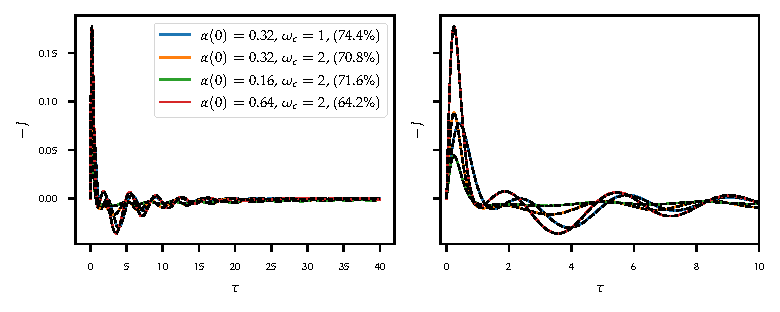
\includegraphics{figs/analytic_comp/flow_comp_nonzero.pdf}
    % \caption{\label{fig:comp_finite_t} The bath energy flow \(-J\) of
    %   the quantum Brownian motion model for different parameters of the
    %   ohmic bath correlation function \cref{eq:ohmic_bcf} in the finite
    %   temperature \(T=1\) case. The presentation is equivalent to
    %   \cref{fig:comp_zero_t}.}
  \end{figure}
\end{frame}

\begin{frame}{Two Baths, Finite Temperature (Gradient)}
  \begin{block}{Parameters}
    \(Ω=Λ=1\), symmetric Ohmic BCFs with
    (\(α(0)=0.25,\, ω_c=2\)), \(N=10^{4}\) samples, \(9\) Hilbert
    space dimensions, \(\ket{ψ(0)}_{\sys} = \ket{0,0}_{\sys}\),
    \(T=0.6\), \(γ=0.5\)
  \end{block}
  \begin{figure}[h]
    \centering
    \begin{subfigure}[t]{.49\linewidth}
      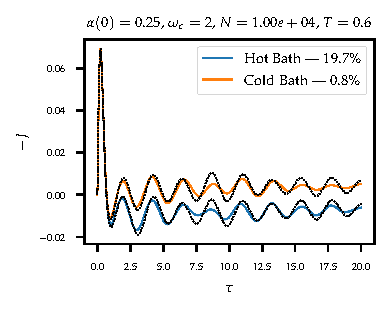
\includegraphics{figs/analytic_comp/comparison_two_5bcf_5ho.pdf}
    \end{subfigure}
    \begin{subfigure}[t]{.49\linewidth}
      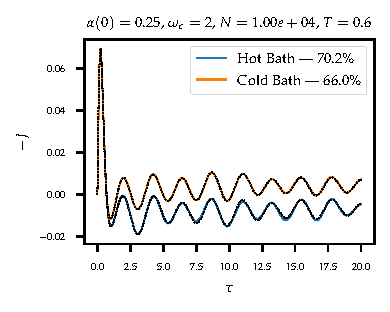
\includegraphics{figs/analytic_comp/comparison_two_ho.pdf}
    \end{subfigure}
  \end{figure}
\end{frame}

% \subsection{First Experiments}
% \begin{frame}{One Qubit, One Bath, Zero Temperature}
%   \begin{columns}
%     \begin{column}{.39\textwidth}
%     \begin{block}{Model}
%       \begin{equation}
%         \label{eq:01model}
%         \begin{aligned}
%           H_\sys &= \frac12 σ_z & L &= \frac12 σ_x & \ket{ψ(0)} &= \ket{\uparrow}
%         \end{aligned}
%       \end{equation}
%       \begin{itemize}
%       \item Ohmic BCF with cutoff frequency
%         \tval{01/cutoff_freq} and
%         scaling \tval{01/bcf_scale}.
%       \item \tval{01/samples} samples
%         \note[item]{the error bars are almost certainly
%           underestimated}
%         \note[item]{interaction energy of similar oom}
%         \note[item]{\(ω_c=2\) is pretty non-Markovian, usual limit \(ω_c\rightarrow\infty\)}
%       \end{itemize}
%     \end{block}
%   \end{column}
%   \begin{column}{.6\textwidth}
%     \only<1>{\plot{01/system_energy}}%
%     \only<2>{\plot{01/flow}}%
%     \only<3>{\plot{01/interaction}
%     }%
%   \end{column}
%   \end{columns}
% \end{frame}

% \begin{frame}{One Qubit, One Bath, Finite Temperature}
%   \begin{columns}
%     \begin{column}{.39\textwidth}
%     \begin{block}{Model}
%       \begin{equation}
%         \label{eq:01model}
%         \begin{aligned}
%           H_\sys &= \frac12 σ_z & L &= \frac12 σ_x & \ket{ψ(0)} &= \ket{\uparrow}
%         \end{aligned}
%       \end{equation}
%       \begin{itemize}
%       \item Ohmic BCF with cutoff frequency \tval{02/cutoff_freq} and
%         scaling \tval{02/bcf_scale}
%       \item Temperature \tval{02/temp}
%       \item \tval{02/samples} samples
%         \note[item]{didn't have many resources, just quick test}
%       % \item<2-> initial gain, then steady loss
%       % \item<3-> gain compensated by interaction
%       \end{itemize}
%     \end{block}
%   \end{column}
%   \begin{column}{.6\textwidth}
%     \only<1>{\plot{02/system_energy}}%
%     \only<2>{\plot{02/flow}}%
%     \only<3>{\plot{02/interaction}}%
%   \end{column}
%   \end{columns}
% \end{frame}

% \begin{frame}
%   \begin{center}
%     Consistency check with interaction energy is difficult and not
%     totally conclusive.

%     \note[item]{convergence..., only indirect,
%       numerical integration}

%     \pause \(\implies\) Analytic Verification
%   \end{center}
% \end{frame}

\section{Applications}

\subsection{One Bath}
\begin{frame}
  \frametitle{One Bath, Zero Temperature}
  \begin{block}{Model: Spin-Boson}
    \begin{equation}
      \label{eq:one_qubit_model}
      H = \frac{1}{2} σ_z + \frac{1}{2} ∑_λ\qty(g_λ σ_x^† a_λ + g_λ^\ast
      σ_x a_λ^†) + ∑_λ ω_λ a_λ^\dag a_λ,\;\ket{ψ_{0}}_{\sys} = \ket{\uparrow}
    \end{equation}
  \end{block}
  \begin{itemize}
  \item<+-> how do we check convergence:\pause
    \begin{itemize}
    \item old: difference of results to some ``good'' configuration\pause
    \item new: consistency with energy conservation
    \end{itemize}
  \end{itemize}
\end{frame}

\begin{frame}
  \frametitle{Example: Dependence of the Interaction Energy on Stochastic Process
    Sampling}
  \begin{figure}[h]
    \centering
    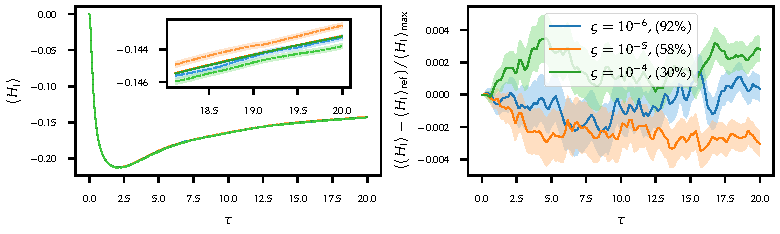
\includegraphics{figs/one_bath_syst/stocproc_systematics_interaction}
  \end{figure}
  \begin{itemize}
  \item \(α(0)=1.6\) and \(ω_{c}=4\) \(\implies\) stress HOPS through
    fast decaying BCF
  \item ``perfect'' results only with very high
    accuracy\footnote{smaller \(\varsigma\) is better} \(\varsigma\)
  \item good qualitative results for less extreme configurations
    (common theme)
  \end{itemize}
\end{frame}

\begin{frame}
  \frametitle{Various Cutoff Frequencies}
  \begin{figure}[h]
    \centering
    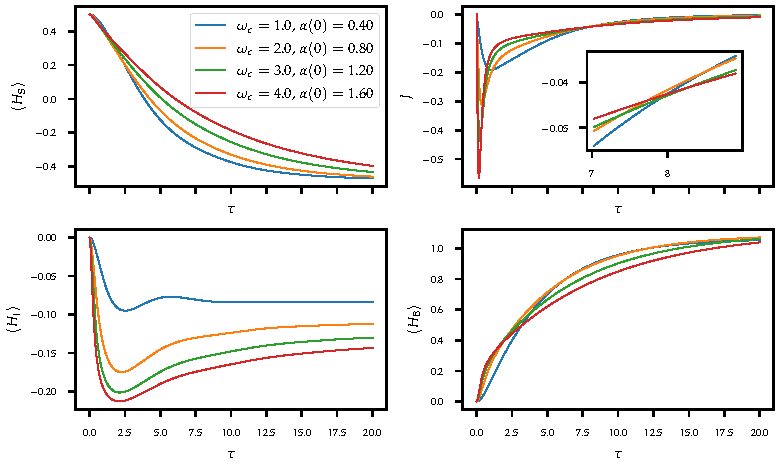
\includegraphics[height=.9\textheight]{figs/one_bath_syst/omega_energy_overview}
    \note[item]{marked differences between trajcetories -> non-markov,
      strong coup}
  \end{figure}
\end{frame}

\begin{frame}{Non-Markovian Dynamics}
  \begin{figure}[h]
    \centering
    \only<1>{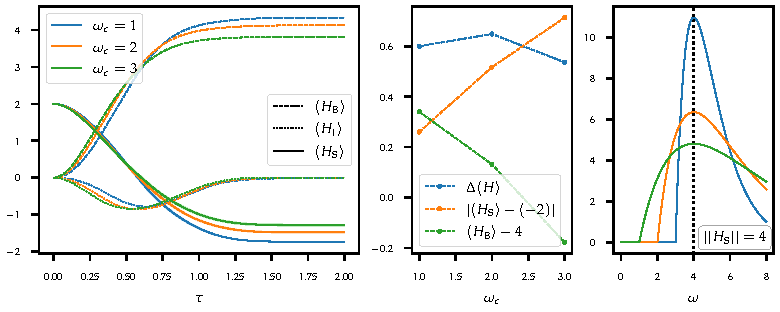
\includegraphics{figs/one_bath_syst/markov_analysis}}
    \only<2>{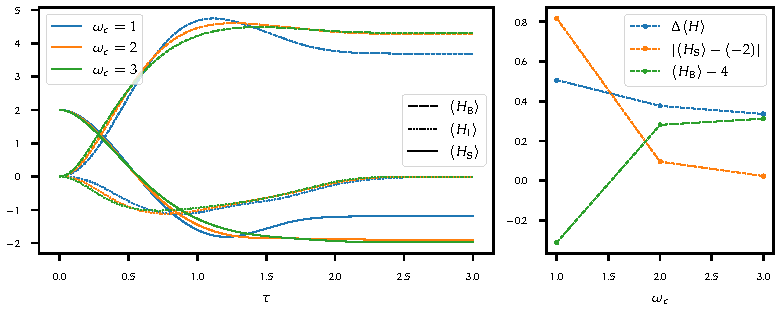
\includegraphics{figs/one_bath_syst/markov_analysis_longer}}
  \end{figure}
  \begin{itemize}
  \item<+-> interaction strengths chosen for approx. same interaction
    energy
  \item<+-> timing important for energy transfer ``performance''
  \end{itemize}
\end{frame}

\begin{frame}
  \begin{center}
    \begin{alertblock}{Beware :)}
      The following is WIP and has not been written up properly yet.
    \end{alertblock}
  \end{center}
\end{frame}


\subsection{Energy Shovel}
\begin{frame}
  \frametitle{Extracting Energy from One Bath}
  \begin{itemize}
  \item same model as above \cref{eq:one_qubit_model}, but with \(L(τ) =
    \sin^2(\frac{Δ}{2} τ)σ_x\)
  \item how much energy can be \emph{unitarily} extracted?
    \(\implies\) \(ΔE_{\mathrm{max}}=\frac{1}{β}\qrelent{ρ_{\sys}}{ρ_{\sys}^{β}}\)
  \end{itemize}
  \begin{figure}[h]
    \centering
    \only<1>{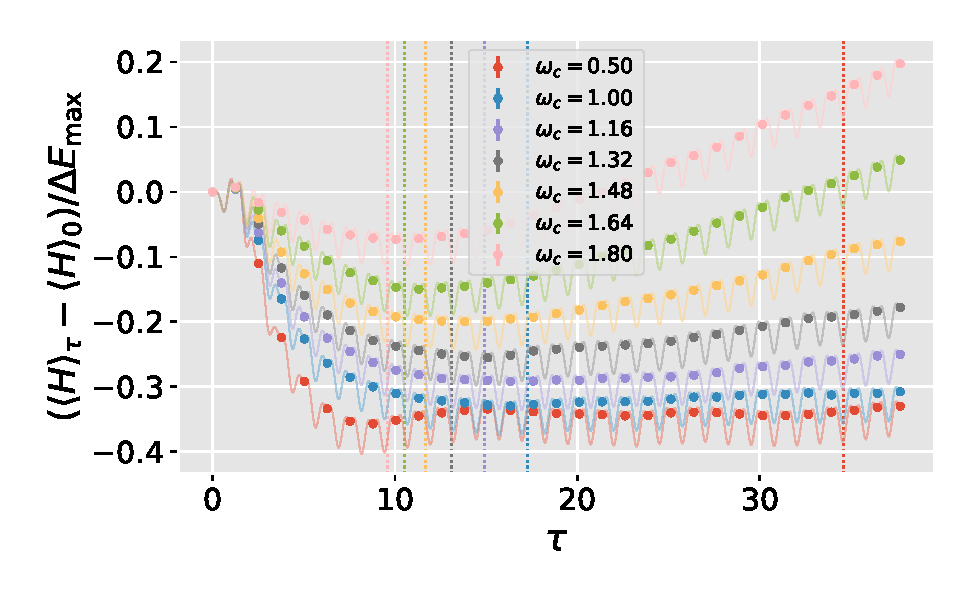
\includegraphics[height=.65\textheight]{figs/modcoup/omegas_total}}
    \only<2>{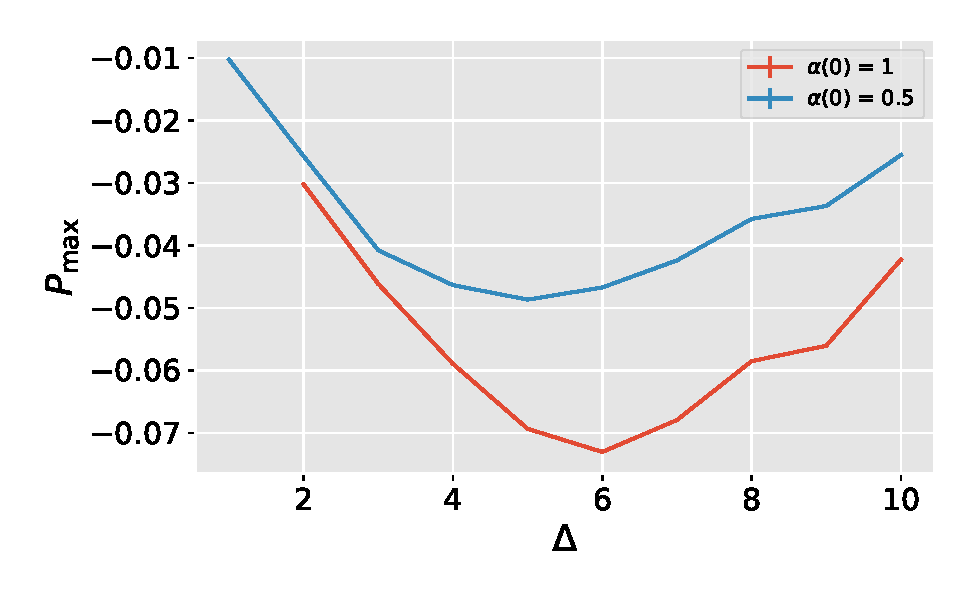
\includegraphics[height=.65\textheight]{figs/modcoup/delta_dependence}}
  \end{figure}
  \note[item]{energy normalized to ergo}
  \note[item]{vert lines bath memory time}
\end{frame}


\subsection{Otto Cycle}
\begin{frame}
  \frametitle{Otto Cycle (proof of concept)}
  \begin{block}{Model}
    Spin-Boson model with compression of \(H_{\sys}\) and modulation
    of \(L\).
  \end{block}
  \begin{itemize}
  \item classical toy model of the quantum heat engine community\footcite{Geva1992Feb}
  \end{itemize}
  \begin{figure}[h]
    \centering
    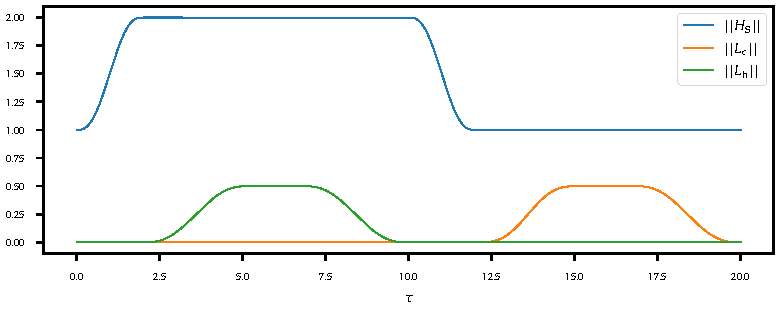
\includegraphics{figs/otto/modulation}
  \end{figure}
\end{frame}
\begin{frame}
  \begin{figure}[h]
    \centering
    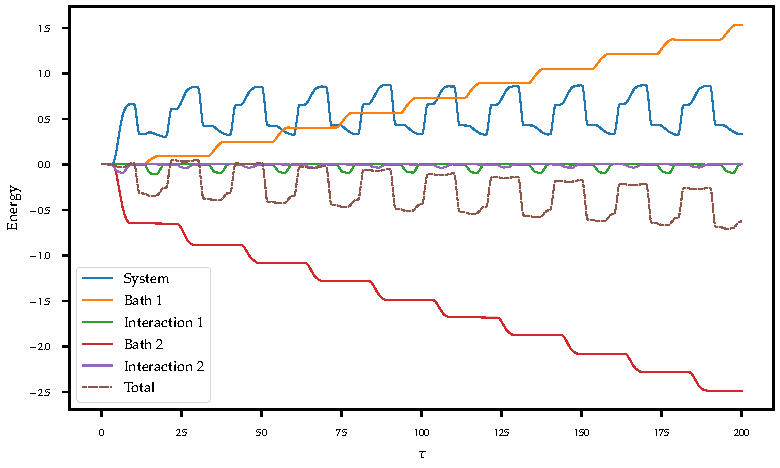
\includegraphics{figs/otto/energy_cont}
  \end{figure}
\end{frame}
\begin{frame}
  \begin{figure}[h]
    \centering
    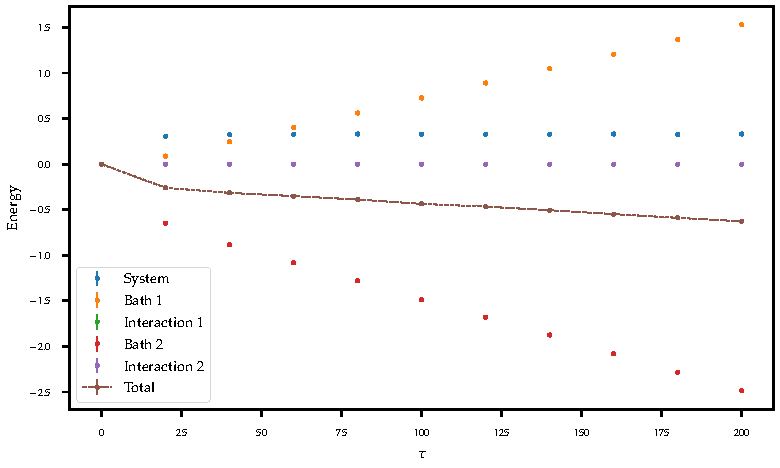
\includegraphics{figs/otto/energy_strobe}
  \end{figure}
\end{frame}
\begin{frame}
  \begin{figure}[h]
    \centering
    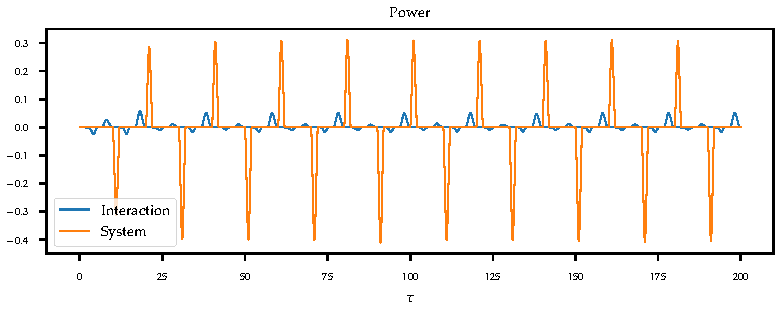
\includegraphics{figs/otto/power}
  \end{figure}
  \begin{itemize}
  \item \(\bar{P} = 1.98 \cdot 10^{-3} \pm 2.3 \cdot 10^{-5}\),
    \(η\approx 20\%\), \(T_{c}=1\), \(T_{h}=20\)
  \item no tuning of parameters, except for resonant coupling
  \item long bath memory \(ω_{c}=1\), but weak-ish coupling
  \end{itemize}
\end{frame}
\begin{frame}{Questions (for the future)}
  \begin{itemize}
  \item better performance through ``overlapping'' phases?
  \item strong coupling any good?
  \item non-Markovianity + strong coupling any good?
  \item what is the optimal efficiency and power? (probably no
    advantage here)
  \end{itemize}
\end{frame}

\subsection{Anti-Zeno Engine}
\begin{frame}
  \frametitle{Anti-Zeno Engine}
  \begin{block}{Question}
    Is there a use for non-Markovianity in quantum heat engines?
  \end{block}
  \begin{itemize}
  \item \cite{Mukherjee2020Jan} claims that one can exploit the
    time-energy uncertainty for quantum advantage\footnote{I'd be
      careful to call this quantum advantage.}
  \end{itemize}

  \begin{block}{Model}
    Qubit coupled to two baths of different
      temperatures (\(T_c, T_h\))
      \begin{equation}
        \label{eq:antizenomodel}
        H_\sys= \frac12  \qty[ω_0 + γ Δ\sin(Δ t)]σ_z,\, L_{c,h}=\frac12 σ_x
      \end{equation}
      \note[item]{frictionless dynamics}
  \end{block}
\end{frame}

\begin{frame}
    \begin{figure}[h]
    \centering
    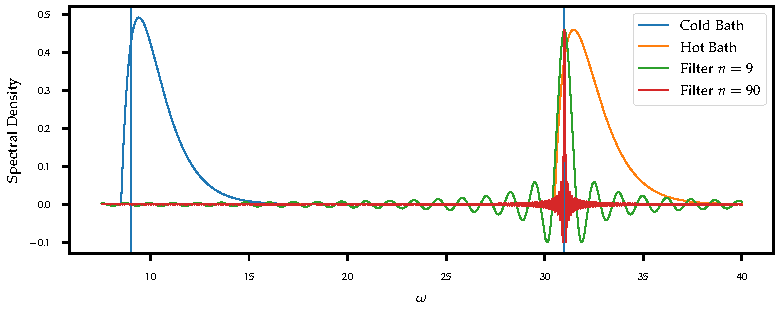
\includegraphics{figs/anti_zeno/with_gap_coupling_diagram}
  \end{figure}
  \begin{itemize}
  \item couple for \(n\) modulation periods slightly of resonance
  \item for smaller \(n\) the \(\sin((ω-(ω_{0}\pm Δ))τ)/((ω-(ω_{0}\pm
    Δ)) τ)\) has a greater overlap
    \(\implies\) controls power output
  \end{itemize}
\end{frame}

\begin{frame}
  \begin{figure}
    \centering
    \begin{subfigure}[t]{.49\linewidth}
      \centering
      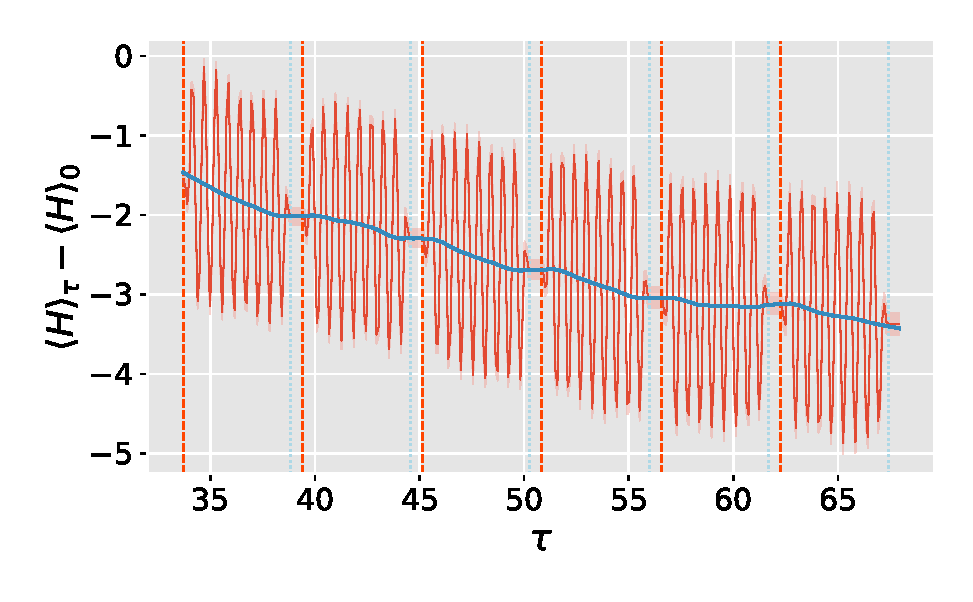
\includegraphics[width=\linewidth]{anti_zeno/anti_zeno_without_cool}
      \caption{\tval{anti_zeno/power_without_cool}}
    \end{subfigure}
    \begin{subfigure}[t]{.49\linewidth}
      \centering
      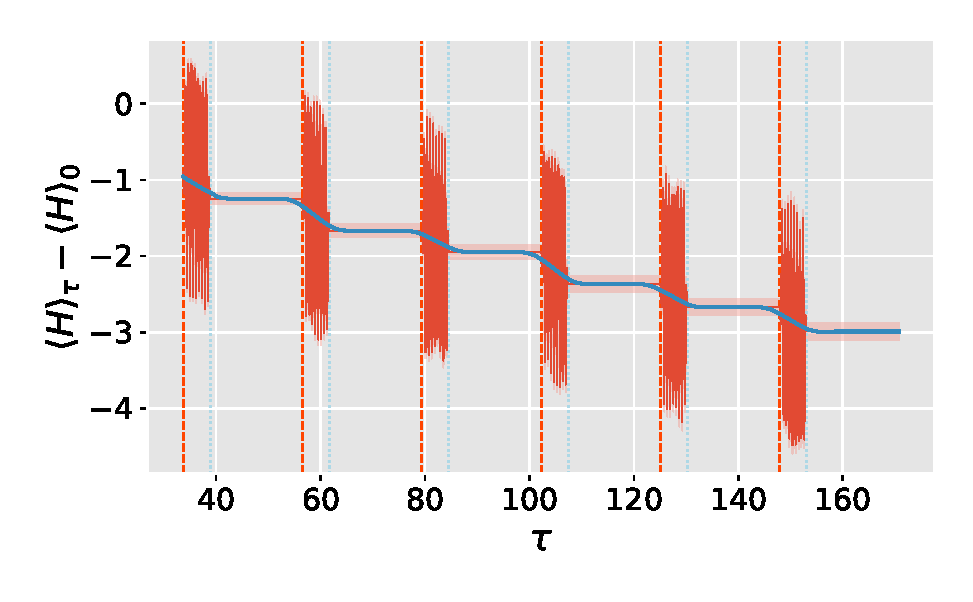
\includegraphics[width=\linewidth]{anti_zeno/anti_zeno_with_cool}
      \caption{
        \tval{anti_zeno/power_with_cool}}
    \end{subfigure}
  \end{figure}
  \begin{exampleblock}{Parameters}
    {\tval{anti_zeno/delta}, \tval{anti_zeno/gamma}, \tval{anti_zeno/omega_alpha},
      \tval{anti_zeno/omega_zero}, \tval{anti_zeno/tc}, \tval{anti_zeno/th}}
  \end{exampleblock}
  \begin{itemize}
  \item this is not properly converged yet \(\rightarrow\) newer
    results: no advantage at these temperatures / coupling strengths
  \item new simulations with temperatures from paper
    (\(β_{h(c)}=0.0005(0.005)\)) are promising
    \begin{itemize}
    \item interesting \(\rightarrow\) no good steady state power in this case
      (insufficient samples?)
    \end{itemize}
  \end{itemize}
\end{frame}


\section{Outlook}
\label{sec:outlook}
\begin{frame}{On the ``To Do'' List}
  \begin{itemize}
  \item verify/falsify weak coupling results in the literature
    (engines)
  \item three-level systems: there is an experimental paper ;)
  \item parameter scan of two qubit model
  \item filter modes
  \item \ldots
  \end{itemize}
\end{frame}

\begin{frame}
  \frametitle{Lessons Learned}
  \begin{itemize}
  \item careful convergence checks pay off
  \item surveying literature is important
  \item properly documenting observations is a great help
    and should be done as early as possible
  \item applications should be carefully chosen to answer interesting
    questions
  \item numerics are helpful, but physical insights are important
  \item comparison with some experiments would have been nice
  \end{itemize}
\end{frame}

\appendix
\begin{frame}[allowframebreaks]{References}
  \printbibliography
\end{frame}

\begin{frame}
  \begin{block}{Situation (Longer)}
    Consider an open quantum system
    \begin{equation}
      \label{eq:openthermo}
      H=\underbrace{H_\sys}_{\text{"small"}}\; +\;
      \underbrace{H_\inter}_{\mathrm{?}} \;+\;
      \underbrace{H_\bath}_{\text{"big", simple}}
    \end{equation}
    with \([H_S, H_B] = 0\).
  \end{block}
  \pause
  \begin{itemize}[<+->]
  \item weak coupling \(H_\inter\approx 0\)
    thermodynamics\footnote{even in strong coupling equilibrium\ldots{}} of open systems
    are somewhat understood \footcite{Rivas2019Oct,Talkner2020Oct}
  \item strong coupling: \(\ev{H_\inter} \sim \ev{H_\sys}\)
    \(\implies\) we can't neglect the interaction \(\implies\)
    thermodynamics?
  \item we do quantum mechanics \(\implies\) can't separate bath
    and system\uncover<+->{, especially not dynamics!}
  \item no consensus about strong coupling thermodynamics:
    \note[item]{won't resolve within scope of masters thesis}
  \item but what is clear: \emph{need to get access to exact dynamics
      of \(H_\inter,H_\bath\)}
  \end{itemize}
\end{frame}

\begin{frame}
  \frametitle{More Papers on Thermo}
  \cite{Rivas2019Oct,Talkner2020Oct,Motz2018Nov,Wiedmann2020Mar,Senior2020Feb,Kato2015Aug,Kato2016Dec,Strasberg2021Aug,Talkner2016Aug,Bera2021Feb,Bera2021Jun,Esposito2015Dec}
\end{frame}

\begin{frame}{Ohmic SD BCF}
  \begin{columns}
    \begin{column}{.49\textwidth}
      \plot{01/ohmic_sd}
    \end{column}
    \begin{column}{.49\textwidth}
      \plot{01/ohmic_bcf}
    \end{column}
  \end{columns}
\end{frame}
\begin{frame}{NMQSD (Zero Temperature)}
  Expanding in a Bargmann (unnormalized) coherent state basis~\cite{klauder1968fundamentals}
  \(\qty{\ket{\vb{z}^{(1)},\vb{z}^{(2)},\ldots}=
    \ket{\underline{\vb{z}}}}\)

  \begin{equation}
    \label{eq:projected}
    \ket{ψ(t)} = ∫∏_{n=1}^N{\qty(\frac{\dd{\vb{z}\nth}}{π^{N_n}}\eu^{-\abs{\vb{z}}^2})}\ket{ψ(t,\underline{\vb{z}}^\ast)}\ket{\underline{\vb{z}}},
  \end{equation}
  we obtain
  \note[item]{interpret the integral in a montecarlo sense}
  \begin{equation}
    \label{eq:multinmqsd}
    ∂_tψ_t(\vb{η}^\ast_t) = -\iu H ψ_t(\vb{η}^\ast_t) +
    \vb{L}\cdot\vb{η}^\ast_tψ_t(\vb{η}^\ast_t) - ∑_{n=1}^N L_n^†∫_0^t\dd{s}α_n(t-s)\fdv{ψ_t(\vb{η}^\ast_t)}{η^\ast_n(s)},
  \end{equation}
  with
  \begin{equation}
    \label{eq:processescorr}
    \begin{aligned}
      \mathcal{M}(η^\ast_n(t)) &=0, & \mathcal{M}(η_n(t)η_m(s)) &= 0,
      & \mathcal{M}(η_n(t)η_m(s)^\ast) &= δ_{nm}α_n(t-s),
    \end{aligned}
  \end{equation}
  where
  \(α_n(t-s)=∑_λ\abs{g_λ\nth}^2\eu^{-\iu
    ω_λ\nth(t-s)}=\ev{B(t)B(s)}_{I,ρ(0)}\) \cite{Strunz2001Habil}
  (fourier transf. of spectral density
  \(J(ω) = π ∑_λ\abs{g_λ}^2δ(ω-ω_λ)\)).
\end{frame}
\begin{frame}{Fock-Space Embedding}
  As in \refcite{Gao2021Sep} we can define
  \begin{equation}
    \label{eq:fockpsi}
    \ket{Ψ} = \sum_\kmat\ket{\psi^\kmat}\otimes \ket{\kmat}
  \end{equation}
  where
  \(\ket{\kmat}=\bigotimes_{n=1}^N\bigotimes_{μ=1}^{N_n}\ket{\kmat_{n,μ}}\)
  are bosonic Fock-states.

  Now \cref{eq:multihops} becomes
  \begin{equation}
    \label{eq:fockhops}
    ∂_t\ket{Ψ} = \qty[-\iu H_\sys + \vb{L}\cdot\vb{η}^\ast -
    ∑_{n=1}^N∑_{μ=1}^{M_n}b_{n,μ}^\dag b_{n,μ} W\nth_μ +
    \iu ∑_{n=1}^N∑_{μ=1}^{M_n} \sqrt{G_{n,μ}} \qty(b^†_{n,μ}L_n + b_{n,μ}L^†_n)] \ket{Ψ}.
  \end{equation}
  \pause
  \(\implies\) possible to derive an upper bound for the norm of
  \(\ket{\psi^\kmat}\) \pause \(\implies\) new truncation scheme
  \note[item]{looks somewhat like a non-hermitian hamiltonian}
\end{frame}
\end{document}

\begin{frame}{Multiple Baths}
  \begin{itemize}
  \item theory generalizes easily to \(N\) baths
  \item generalized our HOPS code to \(N\) baths
    \note[item]{added docstrings and typehints to (almost) everything}
    \note[item]{added (some tests) and CI that ensures they aren't broken}
  \item solving a model with two coupled HOs is now possible
    \note[item]{but with much anguish, root precision, bcf fit!!}
    \begin{equation}
      \label{eq:hamiltonian}
      \begin{aligned}
        H &= ∑_{i\in\qty{1,2}} \qty[H^{(i)}_O + q_iB^{(i)} + H_B^{(i)}] + \frac{γ}{4}(q_1-q_2)^2,
      \end{aligned}
    \end{equation}
    where \(H_O^{(i)}= \frac{Ω_i}{4}\qty(p_i^2+q_i^2)\), \(B^{(i)}=\sum_λ\qty(g^{(i),\ast}_λb^{(i)}_λ  + g^{(i)}_λ
    b^{(i),†}_λ)\) and \(H_B^{(i)}=\sum_λ\omega_λ b^{(i),†}_λ b^{(i)}_λ\).
  \end{itemize}
\end{frame}

\section{Other Projects}
\begin{frame}[allowframebreaks]
  \begin{itemize}
  \item stabilized normalization in nonlinear HOPS
    \begin{figure}
      \centering
      \plot{05/norm}
    \end{figure}
  \item stochastic process sampling via Cholesky decomposition
    \note[item]{allows to generate processes that match up to a point in
      time}
    \note[item]{allows to extend stochastic processes to arbitrary times}
    \note[item]{could be useful for steady state studies and long-time
      propagation}
    \begin{figure}
      \centering
      \plot{05/cholesky}
    \end{figure}
  \item norm based truncation scheme
    \begin{itemize}
    \note[item]{needs further investigation}
    \item promising at ``friendly'' coupling strengths
    \end{itemize}
    \begin{figure}
      \centering
      \plot{06/convergence}
    \end{figure}
  \end{itemize}
\end{frame}


%%% Local Variables:
%%% mode: latex
%%% TeX-master: t
%%% TeX-output-dir: "output"
%%% TeX-engine: luatex
%%% End:
